%%%%%%%%%%%%%%%%%%%%%%%%%%%%%%%%%%%%%%%%%
% Programming/Coding Assignment
% LaTeX Template
%
% This template has been downloaded from:
% http://www.latextemplates.com
%
% Original author:
% Ted Pavlic (http://www.tedpavlic.com)
%
% Note:
% The \lipsum[#] commands throughout this template generate dummy text
% to fill the template out. These commands should all be removed when 
% writing assignment content.
%
% This template uses a Perl script as an example snippet of code, most other
% languages are also usable. Configure them in the "CODE INCLUSION 
% CONFIGURATION" section.
%
%%%%%%%%%%%%%%%%%%%%%%%%%%%%%%%%%%%%%%%%%

%----------------------------------------------------------------------------------------
%	PACKAGES AND OTHER DOCUMENT CONFIGURATIONS
%----------------------------------------------------------------------------------------

\documentclass{article}

\usepackage{fancyhdr} % Required for custom headers
\usepackage{lastpage} % Required to determine the last page for the footer
\usepackage{extramarks} % Required for headers and footers
\usepackage[usenames,dvipsnames]{color} % Required for custom colors
\usepackage{graphicx} % Required to insert images
\usepackage{listings} % Required for insertion of code
\usepackage{courier} % Required for the courier font
\usepackage{lipsum} % Used for inserting dummy 'Lorem ipsum' text into the template
\usepackage[utf8]{inputenc}
\usepackage[ngerman]{babel}
\usepackage{minted}

% Margins
\topmargin=-0.45in
\evensidemargin=0in
\oddsidemargin=0in
\textwidth=6.5in
\textheight=9.0in
\headsep=0.25in

\linespread{1.1} % Line spacing

% Set up the header and footer
\pagestyle{fancy}
%\lhead{\hmwkAuthorName} % Top left header
\chead{\hmwkClass\ : \hmwkTitle} % Top center head
\rhead{\firstxmark} % Top right header
\lfoot{\lastxmark} % Bottom left footer
\cfoot{} % Bottom center footer
\rfoot{Page\ \thepage\ of\ \protect\pageref{LastPage}} % Bottom right footer
\renewcommand\headrulewidth{0.4pt} % Size of the header rule
\renewcommand\footrulewidth{0.4pt} % Size of the footer rule

\setlength\parindent{0pt} % Removes all indentation from paragraphs

%----------------------------------------------------------------------------------------
%	CODE INCLUSION CONFIGURATION
%----------------------------------------------------------------------------------------

\definecolor{MyDarkGreen}{rgb}{0.0,0.4,0.0} % This is the color used for comments
\lstloadlanguages{Perl} % Load Perl syntax for listings, for a list of other languages supported see: ftp://ftp.tex.ac.uk/tex-archive/macros/latex/contrib/listings/listings.pdf
\lstset{language=Perl, % Use Perl in this example
        frame=single, % Single frame around code
        basicstyle=\small\ttfamily, % Use small true type font
        keywordstyle=[1]\color{Blue}\bf, % Perl functions bold and blue
        keywordstyle=[2]\color{Purple}, % Perl function arguments purple
        keywordstyle=[3]\color{Blue}\underbar, % Custom functions underlined and blue
        identifierstyle=, % Nothing special about identifiers                                         
        commentstyle=\usefont{T1}{pcr}{m}{sl}\color{MyDarkGreen}\small, % Comments small dark green courier font
        stringstyle=\color{Purple}, % Strings are purple
        showstringspaces=false, % Don't put marks in string spaces
        tabsize=5, % 5 spaces per tab
        %
        % Put standard Perl functions not included in the default language here
        morekeywords={rand},
        %
        % Put Perl function parameters here
        morekeywords=[2]{on, off, interp},
        %
        % Put user defined functions here
        morekeywords=[3]{test},
       	%
        morecomment=[l][\color{Blue}]{...}, % Line continuation (...) like blue comment
        numbers=left, % Line numbers on left
        firstnumber=1, % Line numbers start with line 1
        numberstyle=\tiny\color{Blue}, % Line numbers are blue and small
        stepnumber=5 % Line numbers go in steps of 5
}

% Creates a new command to include a perl script, the first parameter is the filename of the script (without .pl), the second parameter is the caption
\newcommand{\perlscript}[2]{
\begin{itemize}
\item[]\lstinputlisting[caption=#2,label=#1]{#1.pl}
\end{itemize}
}

%----------------------------------------------------------------------------------------
%	DOCUMENT STRUCTURE COMMANDS
%	Skip this unless you know what you're doing
%----------------------------------------------------------------------------------------

% Header and footer for when a page split occurs within a problem environment
\newcommand{\enterProblemHeader}[1]{
%\nobreak\extramarks{#1}{#1 continued on next page\ldots}\nobreak
%\nobreak\extramarks{#1 (continued)}{#1 continued on next page\ldots}\nobreak
}

% Header and footer for when a page split occurs between problem environments
\newcommand{\exitProblemHeader}[1]{
%\nobreak\extramarks{#1 (continued)}{#1 continued on next page\ldots}\nobreak
%\nobreak\extramarks{#1}{}\nobreak
}

\setcounter{secnumdepth}{0} % Removes default section numbers
\newcounter{homeworkProblemCounter} % Creates a counter to keep track of the number of problems

\newcommand{\homeworkProblemName}{}
\newenvironment{homeworkProblem}[1][Problem \arabic{homeworkProblemCounter}]{ % Makes a new environment called homeworkProblem which takes 1 argument (custom name) but the default is "Problem #"
\stepcounter{homeworkProblemCounter} % Increase counter for number of problems
\renewcommand{\homeworkProblemName}{#1} % Assign \homeworkProblemName the name of the problem
\section{\homeworkProblemName} % Make a section in the document with the custom problem count
\enterProblemHeader{\homeworkProblemName} % Header and footer within the environment
}{
\exitProblemHeader{\homeworkProblemName} % Header and footer after the environment
}

\newcommand{\problemAnswer}[1]{ % Defines the problem answer command with the content as the only argument
\noindent\framebox[\columnwidth][c]{\begin{minipage}{0.98\columnwidth}#1\end{minipage}} % Makes the box around the problem answer and puts the content inside
}

\newcommand{\homeworkSectionName}{}
\newenvironment{homeworkSection}[1]{ % New environment for sections within homework problems, takes 1 argument - the name of the section
\renewcommand{\homeworkSectionName}{#1} % Assign \homeworkSectionName to the name of the section from the environment argument
\subsection{\homeworkSectionName} % Make a subsection with the custom name of the subsection
\enterProblemHeader{\homeworkProblemName\ [\homeworkSectionName]} % Header and footer within the environment
}{
\enterProblemHeader{\homeworkProblemName} % Header and footer after the environment
}

%----------------------------------------------------------------------------------------
%	NAME AND CLASS SECTION
%----------------------------------------------------------------------------------------

\newcommand{\hmwkTitle}{Übung\ \#3} % Assignment title
\newcommand{\hmwkDueDate}{Montag,\ 03.\ November\ 2014} % Due date
\newcommand{\hmwkClass}{Reconfigurable Embedded Systems} % Course/class
\newcommand{\hmwkClassTime}{} % Class/lecture time
\newcommand{\hmwkClassInstructor}{} % Teacher/lecturer
\newcommand{\hmwkAuthorName}{Günther Schindler, Sven Dorkenwald, Kilian Bender} % Your name

%----------------------------------------------------------------------------------------
%	TITLE PAGE
%----------------------------------------------------------------------------------------

\title{
\vspace{2in}
\textmd{\textbf{\hmwkClass:\ \hmwkTitle}}\\
\normalsize\vspace{0.1in}\small{Abgabe\ am\ \hmwkDueDate}\\
\vspace{0.1in}\large{\textit{\hmwkClassTime}}
\vspace{3in}
}

\author{\textbf{\hmwkAuthorName}}
\date{} % Insert date here if you want it to appear below your name

%----------------------------------------------------------------------------------------

\begin{document}

\maketitle

%----------------------------------------------------------------------------------------
%	TABLE OF CONTENTS
%----------------------------------------------------------------------------------------

%\setcounter{tocdepth}{1} % Uncomment this line if you don't want subsections listed in the ToC

\newpage
\tableofcontents
\newpage

%----------------------------------------------------------------------------------------
%	PROBLEM 1
%----------------------------------------------------------------------------------------

% To have just one problem per page, simply put a \clearpage after each problem

\begin{homeworkProblem}[LED-Schieberegister]
In der dritten Übung soll der in Übung zwei entwickelte LED-Schieberegister für
das Atlys Entwicklungsboard implementiert werden. Dieser LED-Schieberegister basiert
auf folgendem VHDL-Code.
\begin{minted}{vhdl}
entity led is
  port( clk_deb, clk_in, reset, din: in std_logic;
        LED_REG: out std_logic_vector(3 downto 0));
end led;

architecture Behavioral of led is

signal INT_REG: std_logic_vector(3 downto 0) := (others => '0');
type states is (S0, S1, S2, S3);
signal state: states := S0;
signal clk: std_logic;

begin
  process(clk, reset)
  begin
    if reset = '1' then 
      INT_REG <= (others => '0');
      LED_REG <= (others => '0');
      state <= S0;
    elsif rising_edge(clk) then
      case state is
      when S0 =>
        LED_REG <= INT_REG;
        INT_REG <=  INT_REG(2 downto 0) & din;
        state <= S1;
      when S1 =>
        INT_REG <= INT_REG(2 downto 0) & din;
        state <= S2;
      when S2 =>
        INT_REG <= INT_REG(2 downto 0) & din;
        state <= S3;
      when S3 =>
        INT_REG <= INT_REG(2 downto 0) & din;
        state <= S0;
      end case;
    end if;
  end process;
end Behavioral;
\end{minted}
\end{homeworkProblem}

%----------------------------------------------------------------------------------------
%	Design Properties
%----------------------------------------------------------------------------------------

\begin{homeworkProblem}[Design Properties]
Der erste Schritt einer Implementierung für das Atlys-Board ist die Konfiguration der
Desing Properties in der Xilinx ISE. Aus dem Atlys Reference Manual entnimmt man, dass
es sich um einen Xilinx Spartan-6 LX-45 FPGA handelt. Folglich muss die Family auf
Spartan6 und das Device auf XC65LX45 eingestellt werden. Außerdem kann man dem Reference
Manual entnehmen, dass das 324-pin BGA Package verwendet wird. Dies wird in der Xilinx
ISE durch Auswahl von CSG324 als Package vollzogen.
\begin{center}
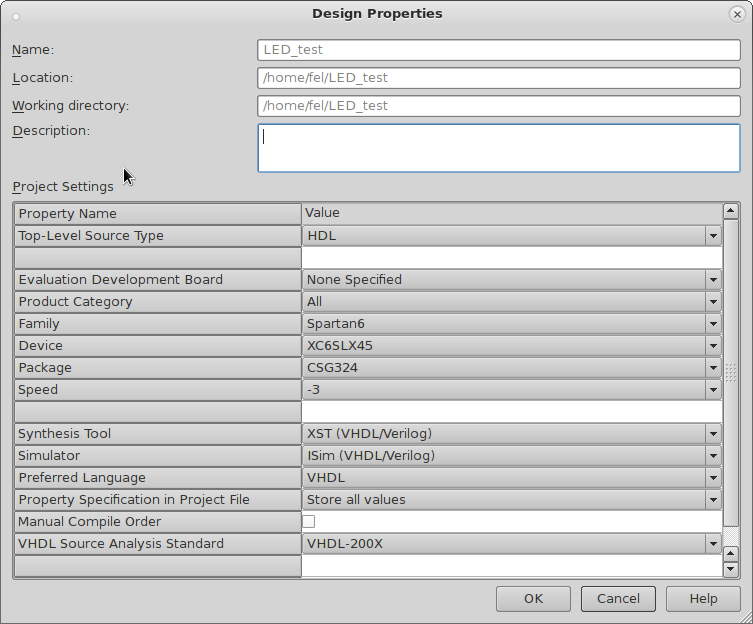
\includegraphics[width=0.5\columnwidth]{designprop}
\end{center}
\end{homeworkProblem}

%----------------------------------------------------------------------------------------
%	Debounce
%----------------------------------------------------------------------------------------

\begin{homeworkProblem}[Debounce]
Als Debounce wird das Entprellen des elektromechanischen Schalters verstanden. Dieser
Schalter ruft bei Betätigung (statt des sofortigen elektrischen Kontakts) kurzzeitig ein
mehrfaches Schließen und Öffnen des Kontakts hervor. Der Grund dieses Prellens sind
Federungen an Bauteilen der Schaltmechanik.
\\
Um diesem physikalischen Effekt entgegenzuwirken wird eine Möglichkeit benötigt,
Schalterbetätigungen mit gewisser Frequenz zu filtern. Dies wird über Verwendung des 
vorgegebenen Debounce VHDL-Codes vorgenommen. Der VHDL-Code muss in das Projekt
eingebunden werden. Die Schalter Prellen mit etwa 1 kHz. Danach wird der Debounce 
bezüglich des LED-Codes wie folgt eingebunden. 
\begin{minted}{vhdl}
...
architecture Behavioral of led is
...
COMPONENT debounce
  PORT(
    clk : IN std_logic;
    rst : IN std_logic;
    din : IN std_logic;          
    dout : OUT std_logic
    );
...
begin
  ...
  Inst_debounce: debounce PORT MAP(
    clk => clk_deb,
    rst => reset,
    din => clk_in,
    dout => clk
    );
  ...
  process(clk, reset)
  begin
  ...
  end process;
end Behavioral;
\end{minted}
\end{homeworkProblem}

%----------------------------------------------------------------------------------------
%	Xilinx-.ucf-File
%----------------------------------------------------------------------------------------

\begin{homeworkProblem}[Xilinx-.ucf-File]
In den Xilinx-.ucf-File (User Constraint File) wird die Verbindung von logischen Netzen
(in- und out-Ports im top level entity) mit physikalischen Pins hergestellt. So gibt es
speziell für das Atlys Board das AtlysGeneral.ucf File, welches alle verwendbaren Pins
enthält. Zusätzlich können auch Timing-Bedingungen abgebildet werden. So wird der auf
dem Atlys Board enthaltene Takt als Referenz Takt für die Debounce-Schaltung verwendet.
\begin{minted}{vhdl}
# clock pin for Atlys rev C board
 NET "clk_deb"   LOC = "L15";

# onBoard Leds
 NET "LED_REG<0>" LOC = "U18";
 NET "LED_REG<1>" LOC = "M14"; 
 NET "LED_REG<2>" LOC = "N14";
 NET "LED_REG<3>" LOC = "L14"; 
 
# onBoard PUSH BUTTONS 
 NET "reset" LOC = "P4";  
 NET "clk_in" LOC = "F6"; 
 
# onBoard SWITCHES
 NET "din" LOC = "A10"; 
\end{minted}
\end{homeworkProblem}

%----------------------------------------------------------------------------------------
%	Testbench
%----------------------------------------------------------------------------------------
\begin{homeworkProblem}[Testbench]
Mit der Testbench wollen wir die korrekte Einbundung und Funktion des Debounce testen.
\\
Über die Konstante clk\_deb\_period setzen wir die Periodendauer auf 10ns und erhalten
über den Prozess clk\_deb\_process einen freilaufenden Takt von 100MHz. Dieser Takt
simuliert den Referenztakt auf dem Atlys-Board. 
\begin{minted}{vhdl}
...
-- Clock period definitions
constant clk_deb_period : time := 10 ns;
...
BEGIN
  ...
  -- Clock process definitions
  clk_deb_process :process
  begin
    clk_deb <= '0';
    wait for clk_deb_period/2;
    clk_deb <= '1';
    wait for clk_deb_period/2;
  end process;
...
END;
\end{minted}
Die Prozedur pulse wird aus der tb\_debounce verwendet um verschiedene Pulsweiten zu 
simulieren. Mit der Prozedur werden die zu entprellenden Signale simuliert.
\begin{minted}{vhdl}
ARCHITECTURE behavior OF tb_led IS 
  ...
  procedure pulse (delay: in natural; signal o: out std_logic) is
  begin
    o <= '0';
    wait for delay * 1000 * clk_deb_period;
    o <= '1';
    wait for delay * 1000 * clk_deb_period;
    o <= '0';
  end procedure;
...
BEGIN
  ...
END;
\end{minted}
Über die doppelte for-Schleife werden je 10 Impulse der Weite 1.0101kHz, 1.000kHz,
0.990kHz und 0.980kHz. Es ist zu erwarten, dass der Debounce die beiden größeren
Frequenzen filtert.
\begin{minted}{vhdl}
ARCHITECTURE behavior OF tb_led IS 
  ...
BEGIN
  ...
  din <= '1';
  l1: for i in 0 to 3 loop
    l2: for j in 0 to 10 loop
      pulse((99 + i), clk_in); 
    end loop;
  end loop;
  ...
END;
\end{minted}
Wie erwartet werden die beiden größeren Frequenzen (bis 40ms) gefiltert. Danach
werden die positiven Taktflanken von din gewertet.
Nach 45ms ist das Ende des 4ten gezählten Zyklus von din erreicht und der
Register wird auf die LEDs geschalten.
\begin{center}
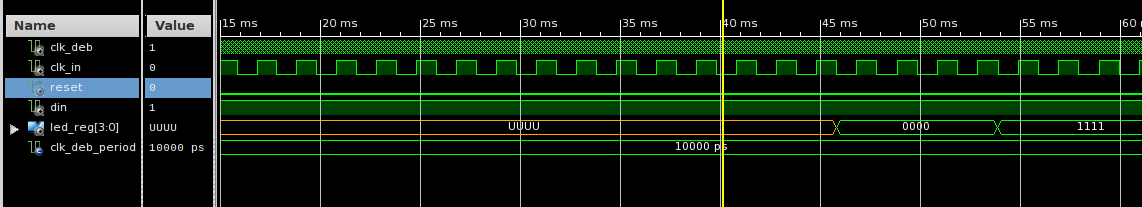
\includegraphics[width=1\columnwidth]{sim}
\end{center}
\end{homeworkProblem}
\clearpage
%----------------------------------------------------------------------------------------

\end{document}